% Diapo des avancements

\begin{frame}[c]
 \frametitle{Hypothesis of simulation}
 \framesubtitle{Structural and dynamics Hypothesis}
 
%  \begin{block}
%  
%   \begin{itemize}
%    \item \tval{E\_cadherin}: has a pulse signal
%    \item We introduce \tval{auto-hit} at the transcription factor level
%    \item We assume that mRNA expression have \tval{three levels of expression}
%   % \item \alert{We now work with the complete graph}
%   \end{itemize}
% 
%  \end{block}

 \begin{columns}
 \begin{column}{0.6\textwidth}
 \begin{tikzpicture}[auto]

\node[qgre] (a1) at (-3,-3) {a};
\node[qgre] (a2) at (-1,-3) {b};
\node[qgre] (a3) at (1,-3) {c};
\node[qgre] (a4) at (3,-3) {d};
%\node[qgre] (a5) at (5,-3) {e};

\node[mod] (i1) at (-3,-2) {};
\node[mod] (i2) at (-1,-2) {};
\node[mod] (i3) at (1,-2) {};
\node[mod] (i4) at (3,-2) {};
%\node[mod] (i5) at (5,-2) {};

\node[ps] (ps1) at (-3,-1) {PS1};
\node[ps] (ps2) at (-1,-1) {PS2};
\node[ps] (ps3) at (1,-1) {PS3};
\node[ps] (ps4) at (3,-1) {PS4};
%\node[ps] (ps5) at (5,-1) {PS5};

\node[mod] (i6) at (-3,0) {};
%\node[mod] (i7) at (-1,0) {};
\node[mod] (i8) at (1,0) {};
\node[mod] (i9) at (3,0) {};
%\node[mod] (i10) at (5,0) {};

\node[ps] (ps6) at (-3,1) {PS6};
%\node[ps] (ps7) at (-1,1) {PS7};
\node[ps] (ps8) at (1,1) {PS8};
\node[ps] (ps9) at (3,1) {PS9};
%\node[ps] (ps10) at (5,1) {PS10};

%les complex
\node[ecad] (d) at (0,3) {Ecad};
\node[cplx] (c1) at (2,-1) {cplx1};
\node[cplx] (c2) at (0,1) {cplx2};
\node[cplx] (c3) at (-2,-1) {cplx3};
\node[cplx] (c4) at (-2,1) {cplx4};
\node[cplx] (c5) at (0,0) {cplx5};
\node[cplx] (c6) at (2,1) {cplx6};

%les seed node
\node[sn] (sn1) at (-2,-3) {SN1};
\node[sn] (sn2) at (2,-3) {SN2};


%les edges 

\path
 (i1) edge[st] (a1)
 (i2) edge[st] (a2)
 (i3) edge[st]  (a3)
 (i4) edge[st]  (a4)
 %(i5) edge[st]  (a5)
 
 (ps1) edge[act] (i1)
 (ps2) edge[act] (i2)
 (ps3) edge[act] (i2)
 (ps3) edge[act] (i3)
 (ps4) edge[act] (i4)
 %(ps5) edge[act] (i5)
 
 (i6) edge[st] (ps1)
 (i6) edge[st] (ps2)
 (i8) edge[st] (ps3)
 (i9) edge[st] (ps4)
 (i9) edge[st] (ps4)
 %(i9) edge[st] (ps5)
 %(i10) edge[st] (ps5)
 
 (ps6) edge[act] (i6)
 (ps8) edge[act] (i8)
 (ps9) edge[act] (i9)
 %(ps10) edge[act] (i10)
 
 (d) edge[act] (ps6)
 (d) edge[act] (ps8)
 (d) edge[act] (ps9)
 %(d) edge[act] (ps10)
 
 (c4) edge[act] (c5)
 (c2) edge[act] (c5)
 (d) edge[act] (c2)
 (c5) edge[inh] (ps2)
 (c6) edge[act] (i8)
 (c6) edge[act] (i9)
 (i8) edge[st] (c1)
 (i9) edge[st] (c1)
 (c1) edge[act] (i4)
 
 (ps3) edge[inh] (sn2)
 (i4) edge[st] (sn2)
 
 (ps1) edge[inh] (sn1)
 (c3) edge[act] (sn1)
 (c4) edge[act] (c3)
 
 (a1) edge[inh, bend left] (ps6);
 

\end{tikzpicture}

\end{column}
\begin{column}{0.4\textwidth}
 \begin{itemize}
   \item \tval{E\_cadherin}: has a pulse signal
   \item We introduce \tval{auto-hit} at the transcription factor level
   \item We assume that mRNA expression have \tval{three levels of expression}
  % \item \alert{We now work with the complete graph}
  \end{itemize}
\end{column}

\end{columns}
 
 
\end{frame}


\begin{frame}[c]
  \frametitle{Simulations and analysis}
  
 \begin{center}
  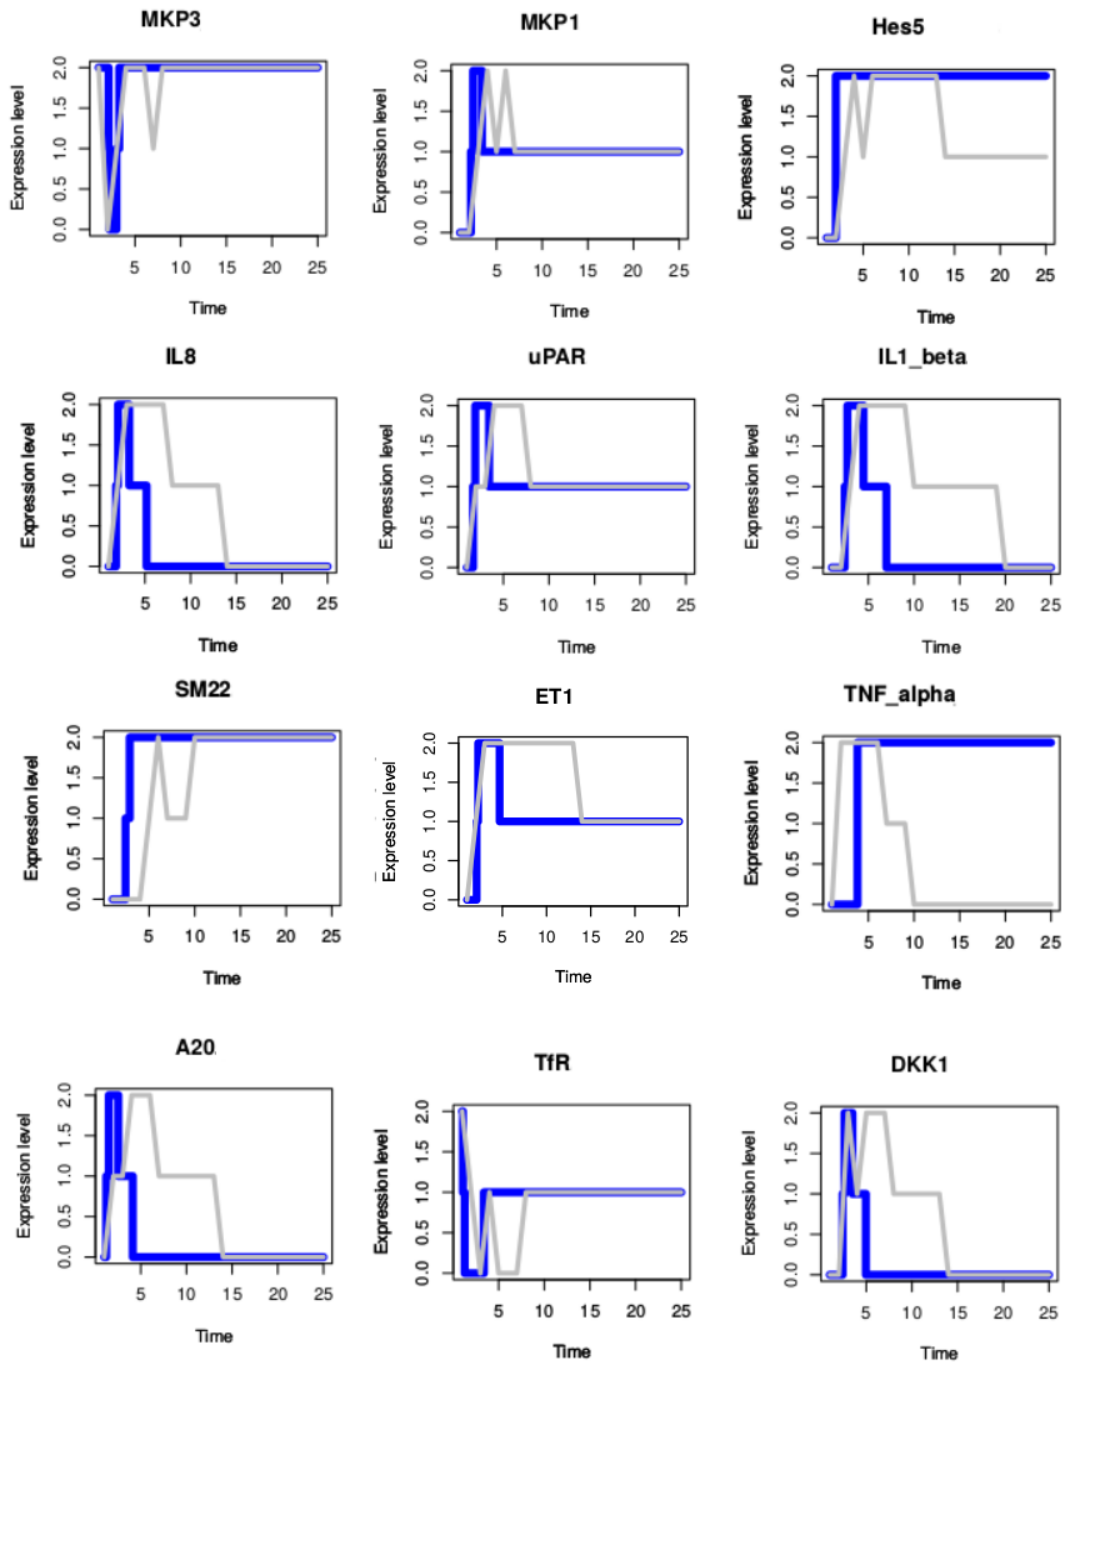
\includegraphics[scale=0.15]{figs/12genes_sim.png}
\end{center}

\textbf{Simulations}

\begin{itemize}
  \item For $r_{a} = r_{i}=10.0$ et $sa = 50 $ for all signalling proteins
  \item With estimated $r$ and $sa$ for MKP3, MKP1, uPAR, Hes5,... according to their expression profiles
  
\end{itemize}

%\textcolor{couleurtheme}{$\Rightarrow$} \fbox{\tval{\large Analyse???}} \textcolor{couleurtheme}{$\Leftarrow$}

\end{frame}




\begin{frame}[c]
  \frametitle{Simulations and analysis}
  
 \begin{center}
  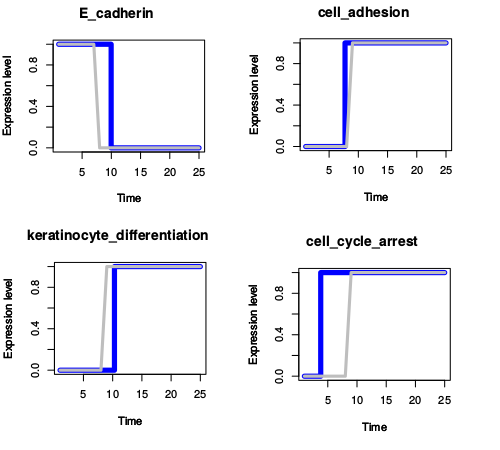
\includegraphics[scale=0.35]{figs/key_nodes1.png}
\end{center}

\textbf{Simulations}

\begin{itemize}
  \item Input node of the system (E\_cadherin)
 \item For biological processes (Cell adhesion, Cell cycle arrest, Keratinocyte differentiation)
  
\end{itemize}

%\textcolor{couleurtheme}{$\Rightarrow$} \fbox{\tval{\large Analyse???}} \textcolor{couleurtheme}{$\Leftarrow$}

\end{frame}
